\thesischapter{Background: Resolution and the Satisfiability Problem}{Background: Resolution and the Satisfiability Problem}
\chaptermark{Resolution and the Satisfiability Problem}
\label{chapter:satbackground}
In the following we shall present the satisfiability problem and  algorithms which solve this problem which are commonly known as SAT solvers. We are particularly interested in the Davis Putnam Logemann Loveland algorithm \cite{DPLL} which is an improvement of the first SAT solving algorithm by Davis and Putnam \cite{MD60}. Moving on from these early SAT algorithms, we shall introduce some more recent SAT algorithms that are improvements on the original DPLL algorithm and include optimisations such as \emph{clause learning}~\cite{MS99} and \emph{non-chronological back tracking} \cite{MM01}. Finally, we look at the resolution algorithm \cite{JR65}, which was directly inspired by the DPLL algorithm, and its associated proof system. The connection between these algorithms is so fundamental  that the DPLL proof system is equivalent to a restricted form of resolution namely \emph{tree resolution} \cite{JR68} and clause learning algorithms have been shown to implement \emph{general resolution} \cite{KP09}. A general introduction to the satisfiability problem and SAT solvers can be found in The Handbook of Satisfiability \cite{AB09b}.


\section{The Satisfiability Problem}
In the following section we will introduce some preliminaries followed by the boolean satisfaction problem, which is the problem of finding a set of assignments to the variables of a formula such that the formula itself becomes true. The majority of modern algorithms for solving this problem work on propositional formulas in \emph{conjunctive normal form}. That is the formula is a conjunction of clauses which are themselves disjunctions of literals. This encoding has the advantage that it has a very simple and structured form making algorithm implementation easier. In order to apply most modern SAT solvers typically one has to first encode the SAT problem as a CNF formula. There are a number of translations available; some naive approaches can exponentially increase the size of the resulting formula. In the following we look at the most commonly used encoding called the Tseitin Expansion \cite{GT83}.
\medskip
\begin{mydef}[Preliminaries]
We define the following preliminaries to use when referring to DPLL SAT algorithms:

\begin{enumerate}
\item A \emph{literal} $l$ is either a positive variable $+v$ or a negative variable $-v$, i.e.\ a variable $v$ with a label $+$ or ${-}$ attached.

\item For every literal $l$ we define the opposite literal $\mybar{l}$ by $\mybar{+v}= -v$, $\mybar{-v} = +v$. 

\item We set $\var{+v} = \var{-v} = v$, $\var{L} = \{\var{l} \mid l\in L\}$
for a set of literals $L$, and 
$\var{\Delta} = \bigcup\{\var{L}\mid L\in\Delta\}$ for a set of sets of 
literals $\Delta$.

\item A \emph{clause} $C$ is a finite set of literals 
$\{ l_1, \ldots , l_k \}$, to be viewed as the disjunction of the literals.

\item A formula in \emph{conjunctive normal form} (CNF) is a 
finite conjunction of clauses. 
%where a clause is a finite disjunction of propositional literals giving it the structure: 
%%
%$$\bigwedge^n_{i=1}(l_1 \vee l_2 \vee \ldots \vee l_{k_i})$$.
%
By a \emph{formula} $\Delta$ we will always mean a formula in CNF,
and we will identify it with a finite set of clauses 
$\{ C_1 , \ldots , C_k \}$, representing the conjunction of the $C_i$.

\item A \emph{valuation} $\Gamma$ is a finite set of literals $\{ l_1, \ldots , l_k \}$ to be viewed as the conjunction of the elements.

\item A valuation $\Gamma$ is \emph{consistent} ($\consistent{\Gamma}$) if 
%
$\forall l \,( l \in \Gamma \to \mybar{l} \notin \Gamma)$.
We let $\consvals$ denote the set of all consistent valuations.


\item A \emph{model} is a total function $M$ which maps literals to booleans and satisfies the property
%
$\forall l \, (M \ l \leftrightarrow \neg M \ \mybar{l})$.
%
\end{enumerate}
%
We shall use the abbreviations 
%
\begin{itemize}
%
\item $M \models \Gamma$, for $\forall l \in \Gamma \, (M \ l)$ 
(`$M$ is a model of $\Gamma$'),
%
\item $M \models \Delta$, for 
$\forall C \in \Delta \, \exists l \in C \,(M \ l)$ 
(`$M$ is a model of $\Delta$').
%
\end{itemize}
%
We call a valuation $\Gamma$ and a formula $\Delta$ \emph{compatible} 
($\compatible{\Gamma}{\Delta})$
if there exists a model satisfying both, i.e. 
$\exists M \, (M \models \Gamma \wedge M\models \Delta)$;
otherwise $\Gamma$ and $\Delta$ are called \emph{incompatible} 
($\incompatible{\Gamma}{\Delta}$).

Note: we will modify some of these definitions in order to make algorithmic improvements.
\end{mydef}

%
%\begin{definition}
A \emph{sequent} $\Gamma \vdash \Delta$ is a pair consisting of a valuation and a formula.
%\end{definition}
%
The intended meaning of a sequent $\Gamma \vdash \Delta$ is that $\Gamma$ and $\Delta$
are incompatible. As a special case, when $\Gamma$ is empty, $\vdash \Delta$ means that $\Delta$ is unsatisfiable. 
\begin{comment}
\begin{defi}
We define an equivalence relation $\sim$ over the formulae $\Delta_1$ and $\Delta_2$ as follows
$$\Delta_1 \sim \Delta_2 \leftrightarrow \forall C .( C \in \Delta_1 \leftrightarrow C \in \Delta_2) $$
\end{defi}
\end{comment}
%
In the following we use the notations $X,a := \{x \mid x\in X \lor x = a\}$ 
(adding $a$ to the set $X$) and 
$X\setminus a := \{x \mid x\in X \land x \neq a\}$ (removing $a$ from $X$).
%
\medskip
\begin{mydef}[The boolean satisfiability (SAT) problem]
Given a formula $\Delta$, does there exist a valuation $\Gamma$ such that:
$$\Gamma \models \Delta$$
\end{mydef}
This is an NP complete problem, meaning that it is solvable by a non-deterministic Turing machine in polynomial time. Such problems are solved by a backtracking search for a potential solution: first an  assignment the variables is tried and if that fails then the algorithm un-does some assignments and tries another solution until all potential solutions have been tried. If all potential solutions do not satisfy the problem then it is said to be unsatisfiable i.e. it has no solution.
\section{The DPLL Algorithm}
The DPLL algorithm attempts to solve the satisfiability problem by performing a search of the problem space. The algorithm consists of a split operation which causes a branching over a literal. The resulting problems in the two sub trees are then simplified using a set of rules before a further branching is applied. Consider the following pigeon hole formula $\mathrm{PHP}(2,1)$ that attempts to put two pigeons into one hole. It is unsatisfiable and therefore the search algorithm branches over the entire space for a result before finally proving that the formula is unsatisfiable.

$$PHP(2,1) := \{\{\neg X_1, \neg X_2\}, \{ X_1 \}, \{ X_2 \} \}$$


\bigskip
\begin{figure}[h!]
\begin{center}
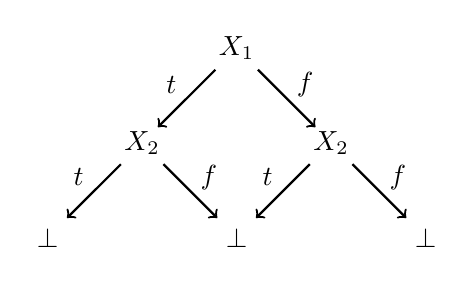
\begin{tikzpicture}
\tikzstyle{arrow}=[->, thick]
\draw node (A)  at (0,0) {$X_1$};
\draw node (B1) at (-1.2,-1.2) {$X_2$};
\draw node (B2) at (1.2,-1.2) {$X_2$};
\draw[arrow] (A) -- node [above = 5pt, left] {$t$} (-1,-1);
\draw[arrow] (A) -- node [above = 5pt, right] {$f$} (1,-1);
\draw node (C1) at (-2.4, -2.4) {$\bot$};
\draw node (C2) at (0, -2.4) {$\bot$};
\draw node (C3) at (2.4, -2.4) {$\bot$};
\draw[arrow] (B1) -- node [above = 5pt, left] {$t$} (C1);
\draw[arrow] (B1) -- node [above = 5pt, right] {$f$} (C2);
\draw[arrow] (B2) -- node [above = 5pt, left] {$t$} (C2);
\draw[arrow] (B2) -- node [above = 5pt, right] {$f$} (C3);


\end{tikzpicture}
\end{center}
\caption{The branching search of the DPLL algorithm, as when applied to PHP(2,1)}
\end{figure}
\bigskip

The DPLL algorithm can be thought of as a recursive function $\mathrm{DPLL}(\Delta,\Gamma)$ which takes a formula and a valuation as input and returns either UNSAT in the case that the formula is unsatisfiable or in the satisfiable case it returns a valuation which forms a model of the formula.  The algorithm begins by applying $\mathrm{Unit-Resolution}$, which repeatedly simplifies the formula by removing clauses that contain a literal in common ($\Red$ Rule, see Definition \ref{def:dpllproofsys}) with the valuation and by removing literals in clauses with opposing literals in the valuation ($\Elim$ Rule, see Definition \ref{def:dpllproofsys}) and then for all resulting \emph{unit} clauses which contain a single literal that literal is added to the valuation ($\Unit$ Rule, see Definition \ref{def:dpllproofsys}).  The algorithm then checks to see if the formula is empty in which case the current valuation forms a satisfying assignment for the formula in which case the algorithm terminates.  Otherwise if this is not the case the algorithms checks to see if the empty clause is in the formula. If the empty clause is in the formula then that clause can not be satisfied and therefore the formula is unsatisfiable with respect to the current valuation and that branch of the algorithm can terminate. If $\mathrm{Unit-Resolution}$ does result in an empty clause then a new literal $l$ is selected from the formula such that neither that literal nor its opposite is in the valuation, then two recursive calls are made, one with the current formula and the valuation extended by $l$ and the second made with the current formula and the valuation extended by the opposite of $l$. 

\begin{lstlisting}[caption = Example DPLL Algorithm,mathescape, label = cl:dpllalg]
DPLL($\Delta, \Gamma$)
$(\Delta, \Gamma) = \mathrm{UnitResolution}(\Delta, \Gamma)$
if $\Delta$ = {} then
	return $\Gamma$
else if {} $\in \Delta$ then
	return UNSAT
else
	$l = \mathrm{Select}(\Delta, \Gamma)$
	if $M$ = DPLL($\Delta, \Gamma \cup \{l\}$) $\neq$ UNSAT then
		return $\Gamma' \cup \Gamma$ 
	else if $M$ = DPLL($\Delta, \Gamma \cup \{\neg l\}$) $\neq$ UNSAT then 
		return $\Gamma' \cup \Gamma$ 
	else
		return UNSAT
\end{lstlisting}

The selection of literals is typically made by some heuristics which are a research topic in their own right and therefore beyond the scope of this thesis. We shall make use of simple heuristics such as  picking the first literal  or choosing the most commonly occurring literal  from a formula as these produce reasonable performance without overly complicating the algorithm or inducing significant overhead.

\subsection*{DPLL Proof System}

The search that this algorithm performs can be viewed as constructing a proof of unsatisfiability for a given formula. The individual operations carried out to during the search correspond to rules in a proof system, which are applied in a backwards fashion. The Unit-Resolution step can be broken down into 3 operations, one that adds unit clauses to the valuation, another that removes clauses that have been satisfied by a literal set to true and finally we have a rule that rules a literal from a clause if its opposing literal is in the valuation. There is an axiom rule $\Conflict$ corresponding to the cases in the algorithm where the empty clause has been derived. Finally, there is a branching rule referred to as $\Split$ which allows a decision to be made on a literal.  The result of an application $\Split$ rule with a literal is two branches; one in which that literal is true in the valuation and another branch in which it is false.
\medskip
\begin{mydef}[DPLL Proof System]\label{def:dpllproofsys} The DPLL proof system consists 
of five rules: 
\label{def:proofsystem-DPLL}
\bigskip \\
%
\begin{center}
%
\AxiomC{$\Gamma, l \vdash \Delta $}
\RightLabel{($\Unit$)}
\UnaryInfC{$\Gamma \vdash \Delta, \{l \} $}
\DisplayProof \
%
\qquad
%
\AxiomC{$\Gamma, l  \vdash \Delta, C$}
\RightLabel{($\Red$)}
\UnaryInfC{$\Gamma, l \vdash \Delta, (C,\mybar{l})$}
\DisplayProof \
%
\qquad
%
\AxiomC{$\Gamma, l \vdash \Delta$}
\RightLabel{($\Elim$)}
\UnaryInfC{$\Gamma, l \vdash \Delta,(C,l)$}
\DisplayProof \

\bigskip

\AxiomC{$$}
\RightLabel{($\Conflict$)}
\UnaryInfC{$\Gamma \vdash \Delta,  \emptyset$}
\DisplayProof \
%
\qquad
%
\AxiomC{$\Gamma,l \vdash \Delta$}
\AxiomC{$\Gamma, \mybar{l} \vdash \Delta$}
\RightLabel{($\Split$)}
\BinaryInfC{$\Gamma  \vdash \Delta$}
\DisplayProof \
%
\end{center}
%
\end{mydef}

There are several variants of the DPLL proof system featured in the literature, the above definition is closest to the Coq formalisation \cite{SL08}, other formalisations such as \cite{FM10b} and \cite{JH09} combine the $\Unit$, $\Red$ and $\Elim$ rules to form a single rule called the "1-literal rule" or "unit propagation".

\section{Conflict Driven Clause Learning Algorithms}
One major improvement to the standard DPLL algorithm is \emph{clause learning} which enables the solvers to learn about the structure of the problem during the proof search, cutting down on the search space in the process. In their most common variant, conflict driven clause learning (CDCL) algorithms, a clause is learned when a conflict is reached that contains the negation of some of the assigned literals that caused the conflict to occur. Typically these algorithms have specialised decision heuristics that take into account the learned clauses.

The first clause learning algorithm was GRASP \cite{MS99,MS96} which exploited the structure of conflicts and learned new clauses during backtracking search. This was greatly improved on by Chaff \cite{LZ01} which included the two watched literal data structure and a heuristic which received feedback from the clause learning process. MiniSAT \cite{NE04} the minimalistic SAT solver takes the optimisations from Chaff and GRASP and tries to structure them in such a way that the SAT solver is easily extended and that one has access to the internal workings of the solver for customisation.

Similarly to the DPLL algorithms, conflict driven clause learning algorithms take as input a formula $\Delta$ in Conjunctive Normal Form. 
A valuation in a clause learning algorithm is typically a total function $\Gamma : \var{\Delta} \to \{0,1,u\}$ that maps to boolean variables of the formula $\Delta$ to a value $0,1$ or $u$ the unassigned value. The depth at which a boolean variable $x$ is assigned a value $\{0,1\}$ in the search tree is called the decision level, which is represented as a function $\delta(x) \in \{-1,0,1, \ldots, |\var{\Delta}| \} $. Instead of removing literals from clauses when they are set to $0$ or removing a clause from the formula when it contains a literal set to $1$ all clauses and their corresponding literals remain in the clause during the search. A mapping $\alpha(x)$ is created associating a boolean variable x with a clause $C$ if that variable is assigned by the unit rule applied to $C$. If a variable $x$ does not have such an antecedent then $\alpha(x) = NIL$.

\subsection*{Conflict Analysis}
The CDCL SAT algorithms cut down on the possible search space for a satisfying assignment by analysing and learning new clauses from conflicts. The causes of the conflict are analysed to see which decision assignments led to the conflict arising. The learned clause contains a negation of these literals such that if it was already in the formula it would have caused the conflict to arise earlier. The decisions and implications that led to the conflict can be seen as forming a graph called a \emph{conflict graph} an example of which can be see in Fig. \ref{fig:conflictgraph}. The literals which are negated to form the learned clause can be seen as forming a bar or cut across the conflict graph. Any of these cuts can be used as learned clauses, however typically the smallest clauses perform better in practice. The majority of modern SAT algorithms try to exploit \emph{unit implication points} (UIP) which are bottlenecks in the conflict graph which form an alternative decision assignment that will cause a conflict in the same clause. Formally a UIP is a dominator in that all paths from the  original decision assignment to the conflict must pass through the UIP node in the graph. 
\medskip
\begin{myexample}
The conflict graph the formula $\phi$ with decisions $x_1 = 1@1$ and $x_7 = 1@2$ is as follows.  The notation $x = 1@n$ means the variable $x$ is assigned to true at $n$ and  $x = 0@n$ means the variable x is assigned to false at level $n$. 
%
\begin{align*}
        \phi &=C_1 \wedge C_2 \wedge C_3 \wedge C_4 \wedge C_5 \wedge C_6 \wedge C_ 7 \wedge C_8\\
               &= (x_1 \vee x_2 \vee x_3) \wedge (\neg x_1 \vee x_4) \wedge (\neg x_2 \vee \neg x_4) \wedge (\neg x_4 \vee x_5) \, \wedge \\
               &\hspace{16pt} (\neg x_3 \vee x_2 \vee  \neg x_5) \wedge (x_2 \vee \neg x_7 \vee x_6) \wedge (\neg x_6 \vee  x_7 \vee x_3) \wedge (\neg x_6 \vee \neg x_7 \vee x_3)
\end{align*}

%
\begin{figure} [H]
\begin{center}
\begin{tikzpicture}[scale = 1.5]
\tikzstyle{box}=[text width = 2cm]
\tikzstyle{arrow}=[->]
\node (A) [box]  at (0,0)                  {\begin{center} $x_1=1@1$ \end{center}};
\node (B) [box]  at (1, 1) 		{\begin{center} $x_4 = 1@1$ \end {center}};
\node (C) [box]  at (2, 2) 		{\begin{center} $x_5 = 1@1$ \end {center}};
\node (D) [box]  at (3, 1) 		{\begin{center} $x_3 = 0@1$ \end {center}};
\node (E) [box]  at (2, 0) 		{\begin{center} $x_2 = 0@1$ \end {center}};
\node (F) [box]  at (4, 0) 		{\begin{center} $\kappa$ \end {center}};
\node (G) [box]  at (3, -1) 		{\begin{center} $x_6 = 1@2$ \end {center}};
\node (H) [box]  at (2, -2) 		{\begin{center} $x_7 = 1@2$ \end {center}};
\draw [arrow] (A) -- node[left] {$C_2$} (B);
\draw [arrow] (B) -- node[left] {$C_3$} (E);
\draw [arrow] (B) -- node[left] {$C_4$} (C);
\draw [arrow] (C) -- node[right] {$C_5$} (D);
\draw [arrow] (E) -- node[below = 2pt, right] {$C_5$} (D);
\draw [arrow] (E) -- node[left] {$C_6$} (G);
\draw [arrow] (H) -- node[left] {$C_6$} (G);
\draw [arrow] (G) -- node[left] {$C_8$} (F);
\draw [arrow] (D) -- node[left] {$C_8$} (F);
\end{tikzpicture} 
\end{center}
\caption{Conflict Graph for the Formula $\phi$}
\label{fig:conflictgraph}

\end{figure}
\end{myexample}

The clause learning process makes use of a resolution operation $\circ$ which resolves two clauses and removes any complimentary literals contained within the two $C_1 \circ C_2 := \{l | l \in C_1 \vee l \in C_2, \neg l \in C_1 \wedge \mybar{l} \in C_2 \}$. The conflict analysis procedure repeatedly applies resolution clauses that are antecedents of the conflict clause. It also makes use of a predicate that computes whether a clause $\omega$ contains an implied literal $l$ that has been assigned at the decision level $d$.

$$\eta(C,l,d) := l \in C \wedge \delta(l) = d \wedge \alpha(l) \neq NIL$$

The conflict analysis procedure takes as input a formula $\Delta$ and a valuation $\Gamma$. It first assigns resulting decision level of the antecedent of the conflict clause to be the end result. It then computes the learned clause by iterating over the antecedents from the conflict clause and resolving them until it is no longer possible to find a literal such that the $\eta$ predicate holds.

\begin{lstlisting}[caption = Conflict Analysis Procedure, mathescape]
ConflictAnalysis($\Delta$,$\Gamma$) 
$i \leftarrow 0$
$\omega \leftarrow \alpha(\kappa)$
$d \leftarrow \omega$
while($\neg \forall l. \eta(\omega,l,d) = 1$)
 do $\omega \leftarrow  \omega \circ \alpha(l)$
$\Delta \leftarrow \Delta \cup \{ \omega \}$
return d
\end{lstlisting}



\subsection*{An Example CDCL Algorithm}

The typical clause learning algorithm functions in a similar way to the DPLL algorithm in that it initially applies unit resolution to the formula. After this it assigns the decision level to zero and then enters a while loop which runs continually until all variables have been assigned. If it manages to assign a value to all of the variables then the current valuation $\Gamma$ can be extended to form a model of the formula $\Delta$. The learned clauses are added to the formula by the $\mathrm{ConflictAnalysis}$ procedure and then cut down on the search space of successive branches of the proof. Even though this algorithm now contains iteration instead of the recursion of the DPLL algorithm (See Code Listing \ref{cl:dpllalg})  it still searches one branch of the search space before backtracking and going down another.




\begin{lstlisting}[caption = Example CDCL Algorithm, mathescape]
CDCL($\Delta$,$\Gamma$)
$(\Delta,\Gamma) = \mathrm{UnitResolution}(\Delta,\Gamma)$
if $\{ \} \in \Delta$
	then return UNSAT
$dl \leftarrow 0$
while($\neg \mathrm{AllVarAssigned}(\Delta,\Gamma$)) do
	do $(x,v) = \mathrm{Select}(\Delta,\Gamma)$
 	     $dl \leftarrow dl + 1$
 	     $\Gamma \leftarrow  \Gamma \cup \{ (x,v)\}$
	     $(\Delta,\Gamma) = \mathrm{UnitResolution}(\Delta,\Gamma)$
	     if $\{ \} \in \Delta$
              	then $\beta = \mathrm{ConflictAnalysis}(\Delta,\Gamma)$
		if $(\beta < 0)$
			then return UNSAT
			else $\mathrm{Backtrack}(\Delta, \Gamma, \beta)$
			        $dl \leftarrow \beta$
return (SAT,$\Gamma$)
\end{lstlisting}


\begin{comment}

Resolution Proof System


\begin{mydef}[Resolution Proof System] The derivable resolution sequents $\Gamma \modres{n} C$ with a derivation of size $n$ are conveniently defined by two rules: Subsumption (or axiom) and resolution.
%
\bigskip

\label{def:resolutionps}
\begin{center}
\AxiomC{\phantom{$\Delta \modres{n} C \vee l$}}
\RightLabel{($\Sub$)  $C \subseteq C'$ }
\UnaryInfC{$\Delta,C \modres{0} C'$}
\DisplayProof
%
\qquad
%
\AxiomC{$\Delta \modres{n} C \vee l$}
\AxiomC{$ \Delta \modres{m} C' \vee \bar{l}$}
\RightLabel{($\Res$)}
\BinaryInfC{$\Delta \modres{n + m + 1} C \vee C'$}
\DisplayProof 
\end{center}
\bigskip
\end{mydef}

\end{comment}

\begin{comment}
\section{Translation to CNF}
In order to apply most modern SAT solvers typically one has to first encode the SAT problem as a CNF formula. There are a number of translations available, some naive approaches can exponentially increase the size of the resulting formula. In the following we look at the most commonly used encoding called the Tseitin Expansion \cite{GT83}.


\section{The Future: Satisfiability Modulo Theory}
More recently a new type of solver has emerged that can deal with first order formulae, these solvers are based on SAT algorithms and include extra theory modules for reasoning about arithmetic,arrays, quantifiers and equality, hence the name \emph{satisfiability modulo theory}.
\end{comment}
